\documentclass[11pt,a4paper]{article}
\usepackage[T1]{fontenc}
\usepackage[utf8]{inputenc}
\usepackage{lmodern}
\usepackage[french,provide=*]{babel}
\usepackage[a4paper,margin=2.3cm]{geometry}
\usepackage{microtype}
\usepackage{amsmath,amssymb}
\usepackage{booktabs,tabularx,array,longtable}
\usepackage{enumitem}
\usepackage{caption}
\usepackage{xcolor}
\usepackage{tikz}
\usetikzlibrary{arrows.meta,positioning,fit,calc}
\usepackage{algorithm}
\usepackage[noend]{algpseudocode}
\usepackage[numbers,sort&compress]{natbib}
\usepackage[hidelinks]{hyperref}
\usepackage{tcolorbox}

\newcommand{\og}{\guillemotleft~}
\newcommand{\fg}{~\guillemotright}
\DeclareMathOperator{\med}{m\acute{e}d}
\DeclareMathOperator{\logit}{logit}
\DeclareMathOperator{\Aire}{Aire}
\floatname{algorithm}{Algorithme}
\algrenewcommand\algorithmicrequire{\textbf{Entrées :}}
\algrenewcommand\algorithmicensure{\textbf{Sorties :}}
\algrenewcommand\algorithmicfor{\textbf{pour}}
\algrenewcommand\algorithmicdo{\textbf{faire}}
\algrenewcommand\algorithmicif{\textbf{si}}
\algrenewcommand\algorithmicthen{\textbf{alors}}
\algrenewcommand\algorithmicelse{\textbf{sinon}}
\algrenewcommand\algorithmicreturn{\textbf{retourner}}
\algrenewcommand\algorithmicforall{\textbf{pour tout}}
\captionsetup{font=small,labelfont=bf,labelsep=period}
\setlist{itemsep=2pt,topsep=4pt}
\renewcommand{\tablename}{Tableau}
\newcolumntype{Y}{>{\raggedright\arraybackslash}X}
\definecolor{accent}{HTML}{B4541A}
\definecolor{quiet}{HTML}{5A5A5A}
\newtcolorbox{decision}[1]{colback=accent!5,colframe=accent!70,boxrule=0.6pt,arc=2pt,left=6pt,right=6pt,top=4pt,bottom=4pt,fonttitle=\bfseries\small,title={#1}}

\title{\textbf{HEXAFIRE : harmonisation des points chauds MODIS et VIIRS\\pour un calendrier de l'activité des feux}\\[4pt]\large Document de recherche et de conception --- version fusionnée}
\author{Équipe HEXAFIRE\\[2pt]\small NASA Space Apps Challenge 2026 --- défi \og Harmonization of MODIS and VIIRS Hot Spots\fg}
\date{Version 2.1 du 13 novembre 2026 (résultats provisoires)}

\begin{document}
\maketitle

\begin{abstract}
\noindent Les satellites observent les feux actifs depuis plus de vingt ans, mais l'archive est partagée entre deux familles de capteurs non comparables. MODIS (Terra et Aqua) couvre la période 2000 à aujourd'hui avec des pixels de 1~km. VIIRS (Suomi NPP, NOAA-20, NOAA-21) détecte depuis 2012 plusieurs fois plus de feux grâce à des pixels de 375~m. Concaténer les deux séries crée une rupture instrumentale qui fausse tendances et anomalies. Ce document fusionne les deux études menées au sein de l'équipe HEXAFIRE et fixe la méthode retenue pour le défi \og Harmonization of MODIS and VIIRS Hot Spots\fg{} du NASA Space Apps Challenge 2026.

Après une revue de la littérature et des méthodes d'harmonisation, nous adoptons un modèle qui exprime les détections VIIRS dans l'unité de MODIS, à occasions d'observation égales. Les occasions d'observation sont calculées à partir des empreintes des passages satellites. La conversion est estimée par une régression logistique conditionnelle qui élimine l'activité réelle des feux. Elle est stratifiée par région, couverture du sol, mois de l'année et période (jour ou nuit), et les strates peu actives sont stabilisées par un estimateur à effets aléatoires. Le produit est une série mensuelle continue depuis novembre 2000, assortie d'un intervalle de prédiction et d'un statut d'observation, et un poids harmonisé est attribué à chaque détection. Une application web statique en fait un calendrier interactif sur une zone libre.

Le critère principal de validation traduit directement l'exigence du défi~: le verdict \og bas / normal / haut\fg{} porté sur un mois ne doit pas dépendre du capteur. Il est mesuré par le $\kappa$ de Cohen sur des années et des régions réservées, et comparé à six méthodes existantes.

\medskip\noindent\textbf{Mots-clés~:} feux actifs, MODIS, VIIRS, harmonisation inter-capteurs, occasions d'observation, régression logistique conditionnelle, FIRMS, calendrier des feux.
\end{abstract}

\begin{decision}{Ce que nous faisons, en six décisions}
\small
\begin{enumerate}[leftmargin=*,itemsep=1pt]
  \item \textbf{Unité de référence~: MODIS.} Les détections VIIRS sont converties en \og équivalent MODIS\fg. L'historique 2002--2020 reste mesuré. Un affichage en \og équivalent VIIRS\fg{} est proposé, sans effet sur les anomalies (section~\ref{sec:reference}).
  \item \textbf{Occasions d'observation calculées} à partir des empreintes des passages (catalogue CMR de la NASA), avec une méthode de repli simplifiée (section~\ref{sec:occasions}).
  \item \textbf{Conversion estimée par régression logistique conditionnelle} par strate, mois de l'année et période jour/nuit, avec stabilisation des petites strates (section~\ref{sec:modele}).
  \item \textbf{Bascule vers VIIRS au 1\textsuperscript{er} janvier 2021}, avant la dérive des orbites de Terra et d'Aqua. Les plateformes VIIRS sont combinées par moyenne pondérée par les occasions.
  \item \textbf{Validation par l'invariance du verdict} ($\kappa$ de Cohen), sur des données réservées, avec comparaison à six méthodes existantes (sections~\ref{sec:validation} et \ref{sec:comparaison}).
  \item \textbf{Application statique}~: moteur Python hors ligne, fichiers en tuiles, aucun serveur (section~\ref{sec:archi}).
\end{enumerate}
\textbf{Reste à décider~:} la couverture géographique (Afrique avec zone témoin, ou monde entier), voir section~\ref{sec:plan}.
\end{decision}

\tableofcontents
\newpage

%====================================================================
\section{Introduction}
%====================================================================

\subsection{Contexte}

Les feux de végétation, qu'il s'agisse de feux de forêt, de feux de savane ou de brûlis agricoles, brûlent chaque année environ $774 \pm 63$ millions d'hectares, soit près de 6\,\% des terres émergées (moyenne 2001--2020 selon GFED5~\cite{chen2023}). Ils émettent en moyenne 3,4~Pg de carbone par an~\cite{vanderwerf2025}. Certains écosystèmes ont besoin de feux périodiques. Toutefois, les changements de fréquence, d'étendue ou d'intensité des feux affectent le climat, la biodiversité, la santé et les biens. Une grande part de l'activité de brûlage est d'origine humaine~: feux agricoles et pastoraux, défrichement, élimination des déchets. En Afrique de l'Ouest, la saison sèche concentre une activité de brûlage très importante, en grande partie agricole et pastorale.

Les gestionnaires de territoires et les services d'intervention ont besoin de savoir \emph{quand} et \emph{où} l'activité de brûlage est habituellement forte, et de reconnaître rapidement une situation inhabituelle. Seule l'observation satellitaire fournit cette information de façon homogène sur de grandes surfaces. Les capteurs infrarouges détectent des pixels anormalement chauds par rapport à leur voisinage~: les \emph{points chauds}, ou feux actifs. Le système FIRMS de la NASA diffuse ces détections pour MODIS depuis novembre 2000 et pour VIIRS depuis 2012~\cite{firms}. Chaque point chaud indique la position du centre du pixel, la date et l'heure du passage, le satellite, un indice de confiance et la puissance radiative du feu (FRP).

Un \emph{calendrier d'activité} présente, pour une zone, le nombre de points chauds par mois et par année. D'un seul regard, il montre la saison des feux, les années exceptionnelles et la situation du mois en cours. Pour être utile, il doit être cohérent sur toute la période~: une différence de couleur entre deux cases doit refléter une différence d'activité, et non un changement de satellite.

\subsection{Le défi}

Le défi \og Harmonization of MODIS and VIIRS Hot Spots\fg{} (thèmes \emph{Earth Science} et \emph{Software}, niveau avancé et intermédiaire) constate que l'archive est \og split across sensors whose data cannot be compared directly\fg~\cite{spaceapps2026}. Il demande une application web qui harmonise ces enregistrements en un calendrier de l'activité des feux fondé sur les points chauds, pour une zone d'intérêt choisie par l'utilisateur.

\subsection{Contributions}

Ce travail apporte cinq contributions~:
\begin{enumerate}
  \item une revue structurée des méthodes d'harmonisation inter-capteurs applicables aux détections de feux (section~\ref{sec:methodes})~;
  \item un modèle de conversion qui tient compte explicitement des occasions d'observation, élimine l'activité inconnue par conditionnement et fournit une incertitude de prédiction (section~\ref{sec:modele})~;
  \item un protocole de validation préenregistré, fondé sur l'invariance du verdict porté sur un mois (section~\ref{sec:validation})~;
  \item un banc de comparaison avec six méthodes existantes réimplémentées sur les mêmes données (section~\ref{sec:comparaison})~;
  \item une architecture et des algorithmes qui rendent le produit consultable dans un navigateur sans serveur (sections~\ref{sec:archi} et \ref{sec:appli}).
\end{enumerate}

\begin{tcolorbox}[colback=gray!5,colframe=gray!50,boxrule=0.5pt,arc=2pt]
\small\textbf{Ce que mesure HEXAFIRE.} Un point chaud n'est pas un incendie, et l'absence de point chaud ne prouve pas l'absence de feu. HEXAFIRE mesure l'activité de brûlage détectable depuis l'espace, de manière cohérente dans le temps. Il ne compte pas les incendies, n'estime pas les surfaces brûlées et ne prévoit pas les feux. Il ne remplace ni un système d'alerte opérationnel ni une vérification sur le terrain. Il ne dit jamais \og aucun feu\fg, mais \og aucun point chaud détecté\fg.
\end{tcolorbox}

%====================================================================
\section{Problématique}\label{sec:probleme}
%====================================================================

\subsection{Une rupture instrumentale}

Un utilisateur qui compte les points chauds d'une région de 2000 à aujourd'hui, en prenant MODIS puis VIIRS, voit le nombre de feux bondir au changement de capteur. Ce saut ne traduit aucun changement de l'activité. Des mesures préliminaires de l'équipe sur une zone d'Afrique de l'Ouest indiquent que VIIRS y détecte 3,5 à 6,3 fois plus de feux que MODIS à occasions d'observation égales. Sans harmonisation, un responsable ne peut pas savoir si la saison est exceptionnelle ou si le satellite est simplement plus sensible. Un mois vide peut aussi traduire une absence de feu ou une absence d'observation. Une comparaison du mois en cours à la médiane historique, calculée sur des comptages bruts, produit alors de fausses alertes.

\subsection{Formulation}

Soit $c$ une cellule d'une grille, $m$ un mois civil et $s$ un capteur. Le nombre de points chauds détectés se décompose en trois facteurs~:
\begin{equation}
  N_{s,c,m} \;=\; \underbrace{\lambda_{c,m}}_{\text{activité}} \;\times\; \underbrace{E_{s,c,m}}_{\text{occasions d'observation}} \;\times\; \underbrace{e^{\alpha_{s}}}_{\text{capacité de détection}}.
  \label{eq:decomp}
\end{equation}
Seule l'activité $\lambda$ intéresse l'utilisateur. Les occasions $E$ dépendent de l'orbite, de la fauchée et des pannes. La capacité de détection dépend de la résolution, de la sensibilité, de l'algorithme, de l'heure de passage et des filtres appliqués. Harmoniser consiste à retirer l'influence des deux derniers facteurs.

L'activité absolue n'est pas observable, car il n'existe aucun recensement au sol de tous les feux depuis 2000. On ne peut donc pas vérifier directement qu'une méthode retrouve le nombre réel de feux. On peut en revanche vérifier ce que le défi exige~: \emph{une fois les données harmonisées, le capteur d'origine ne change plus le verdict porté sur un mois}. Ce critère d'invariance du verdict structure la validation (section~\ref{sec:validation}).

\subsection{Sources d'écart entre capteurs}

\begin{table}[h]
\centering\small
\caption{Origines des écarts de comptage entre capteurs.}
\label{tab:ecarts}
\begin{tabularx}{\linewidth}{>{\raggedright\arraybackslash}p{3.1cm} Y Y}
\toprule
Différence & Effet sur le comptage & Illustration \\
\midrule
Résolution et sensibilité & VIIRS détecte des feux plus petits et en compte davantage & Pixel de 375~m contre 1~km au nadir~\cite{schroeder2014}~; FRP minimale d'environ 0,4~MW contre 2,5 à 17~MW pour MODIS~\cite{fu2020} \\
Géométrie de visée & Le pixel MODIS grandit fortement en bord de fauchée & Facteur 9,7 pour MODIS contre 3,3 pour VIIRS~\cite{giglio2025}~; MODIS perd 67\,\% de ses détections du nadir à 60$^\circ$~\cite{li2018} \\
Couverture & Une zone peut ne pas être vue un jour donné & MODIS laisse des bandes non observées entre ses orbites sous les tropiques~\cite{zheng2026} \\
Heure de passage & L'activité d'un feu varie au cours de la journée & Terra est passé de 10~h~30 à environ 9~h fin 2025, Aqua de 13~h~30 vers la fin d'après-midi~\cite{nsidc} \\
Jour et nuit & L'écart entre capteurs est bien plus grand la nuit & VIIRS 375~m détecte 25 fois plus de pixels de feu de nuit que VIIRS 750~m~\cite{schroeder2014} \\
Arrivée et arrêt des satellites & La somme des détections change brusquement & Suomi NPP a cessé de livrer des données le 2 novembre 2026~\cite{earthdata2026} \\
Pannes et lacunes & Une absence de détection peut être une absence de données & FIRMS publie la liste des jours manquants par capteur~\cite{firmsmissing} \\
Données récentes et archive & Le mois en cours et l'historique ne sont pas produits de la même manière & Le mois en cours provient du flux en temps quasi réel \\
\bottomrule
\end{tabularx}
\end{table}

La figure~\ref{fig:frise} situe les capteurs dans le temps et fait apparaître les périodes qui structurent la méthode.

\begin{figure}[h]
\centering
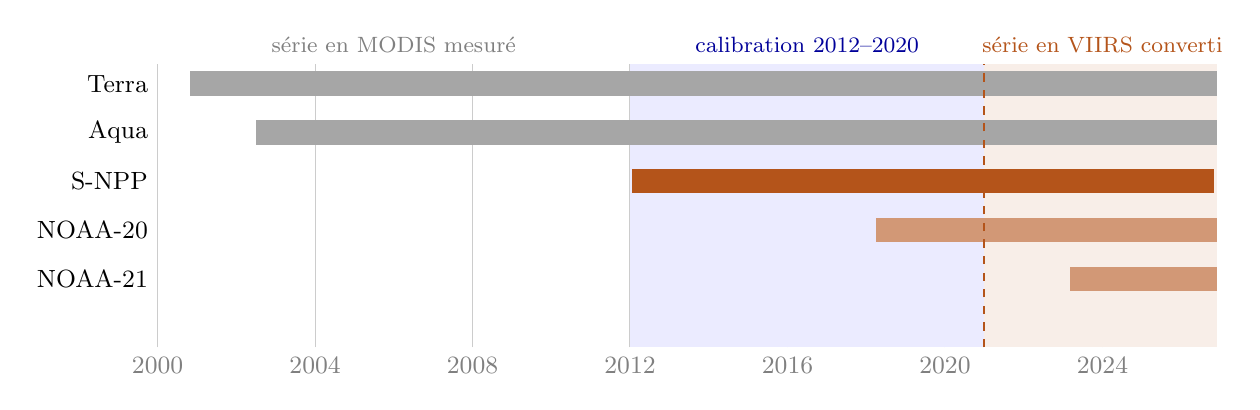
\begin{tikzpicture}[x=0.5cm,y=0.62cm,font=\small]
  \foreach \y in {2000,2004,...,2024} {
    \draw[gray!40] ({\y-2000},-0.4) -- ({\y-2000},5.4);
    \node[below,gray] at ({\y-2000},-0.4) {\y};
  }
  \fill[blue!8] (12,-0.4) rectangle (21,5.4);
  \fill[accent!10] (21,-0.4) rectangle (26.9,5.4);
  \node[blue!60!black,font=\footnotesize] at (16.5,5.8) {calibration 2012--2020};
  \node[accent,font=\footnotesize] at (24,5.8) {série en VIIRS converti};
  \node[gray,font=\footnotesize] at (6,5.8) {série en MODIS mesuré};
  \newcommand{\sbar}[4]{\fill[#4] (#1,#3-0.25) rectangle (#2,#3+0.25);}
  \sbar{0.83}{26.9}{5}{gray!70}   \node[left] at (0,5) {Terra};
  \sbar{2.5}{26.9}{4}{gray!70}    \node[left] at (0,4) {Aqua};
  \sbar{12.05}{26.84}{3}{accent}  \node[left] at (0,3) {S-NPP};
  \sbar{18.25}{26.9}{2}{accent!60}\node[left] at (0,2) {NOAA-20};
  \sbar{23.17}{26.9}{1}{accent!60}\node[left] at (0,1) {NOAA-21};
  \draw[dashed,thick,accent] (21,-0.4) -- (21,5.4);
\end{tikzpicture}
\caption{Disponibilité des capteurs (gris~: MODIS~; orange~: VIIRS 375~m), fenêtre de calibration et bascule de la série vers VIIRS au 1\textsuperscript{er} janvier 2021 (tiretés).}
\label{fig:frise}
\end{figure}

\subsection{Exigences du défi}

Le tableau~\ref{tab:exigences} reprend chaque attente de l'énoncé~\cite{spaceapps2026} et indique où HEXAFIRE y répond.

\begin{longtable}{>{\raggedright\arraybackslash}p{0.8cm} >{\raggedright\arraybackslash}p{5.2cm} >{\raggedright\arraybackslash}p{6.6cm} >{\raggedright\arraybackslash}p{1.4cm}}
\caption{Exigences du défi et réponses d'HEXAFIRE.}\label{tab:exigences}\\
\toprule
N° & Attente de l'énoncé & Réponse d'HEXAFIRE & Section \\
\midrule\endfirsthead
\toprule
N° & Attente de l'énoncé & Réponse d'HEXAFIRE & Section \\
\midrule\endhead
\small E1 & \small Harmoniser pour que \og the sensor of origin no longer matters\fg & \small Conversion de VIIRS dans l'unité MODIS, série unique, test d'invariance du verdict & \small \ref{sec:modele}, \ref{sec:validation} \\
\small E2 & \small Calendrier du \og number of hotspots detected from the early 2000s to the present\fg & \small Calendrier mensuel de novembre 2000 au mois en cours & \small \ref{sec:appli} \\
\small E3 & \small \og Consistent time series\fg{} combinant l'historique MODIS et le détail de VIIRS & \small Série harmonisée avec intervalle, statut d'observation et unité d'affichage au choix & \small \ref{sec:serie} \\
\small E4 & \small Sélectionner une région et une plage de dates & \small Tracé de zone ou saisie de coordonnées, choix de la période & \small \ref{sec:appli} \\
\small E5 & \small Carte interactive, tracé de zone, saisie de latitude et longitude & \small Rectangle, polygone, point avec rayon, emprise en coordonnées & \small \ref{sec:appli} \\
\small E6 & \small Télécharger des analyses et des visualisations & \small Tableaux CSV, figures PNG et SVG, fiche de métadonnées & \small \ref{sec:appli} \\
\small E7 & \small \og CSV file of hot spots detected during a search\fg & \small CSV des détections de la zone et de la période, avec leur poids harmonisé & \small \ref{sec:poids} \\
\small E8 & \small Rampes de couleur accessibles & \small Palettes adaptées aux daltonismes, textures pour les statuts & \small \ref{sec:appli} \\
\small E9 & \small Comparer le mois en cours à l'historique & \small Rapport à la médiane, rang, probabilité de dépassement & \small \ref{sec:indicateurs} \\
\small E10 & \small \og Anomalies against multi-year averages\fg & \small Écart à la moyenne 2003--2020, en valeur et en pourcentage & \small \ref{sec:indicateurs} \\
\small E11 & \small Quelles périodes de l'année voient plus de feux & \small Profil saisonnier~: médiane et quartiles par mois & \small \ref{sec:indicateurs} \\
\small E12 & \small Quelles années ont eu le plus d'activité & \small Classement des années complètes & \small \ref{sec:indicateurs} \\
\small E13 & \small Comment un feu actuel se compare aux précédents & \small Saison en cours et épisode en cours comparés aux précédents & \small \ref{sec:indicateurs} \\
\small E14 & \small Nombre de feux détectés et signalés & \small Points chauds détectés et harmonisés~; les feux signalés au sol ne sont pas disponibles de façon homogène, ce que l'application précise & \small \ref{sec:appli} \\
\small E15 & \small Quelques indices et chiffres clés & \small Quatre indicateurs en tête d'écran & \small \ref{sec:appli} \\
\small E16 & \small Publics~: alerte précoce, secours, scientifiques, gestionnaires, pompiers & \small Lecture simple par défaut, mode expert, méthode détaillée & \small \ref{sec:appli} \\
\small E17 & \small Données FIRMS de la NASA & \small Archive standard et flux récent FIRMS, métadonnées des passages & \small \ref{sec:donnees} \\
\bottomrule
\end{longtable}

%====================================================================
\section{État de l'art}\label{sec:etat}
%====================================================================

\subsection{Détection des feux actifs par satellite}

La détection des feux actifs repose sur la forte émission des flammes dans l'infrarouge moyen, autour de 4~$\mu$m. L'algorithme contextuel de MODIS (produits MOD14 pour Terra et MYD14 pour Aqua, collections~6 et~6.1, cette dernière ne modifiant que l'étalonnage) compare la température de brillance de chaque pixel de 1~km à celle de son voisinage, et déclare un feu lorsque l'écart dépasse des seuils adaptatifs. Il estime aussi la FRP, liée au taux de combustion de la biomasse. Avec Suomi NPP, l'instrument VIIRS a apporté des bandes infrarouges à 375~m. \citet{schroeder2014} ont adapté l'algorithme MODIS à ces bandes pour créer le produit VNP14IMG. Ils montrent qu'il détecte 3 fois plus de pixels de feu de jour et 25 fois plus de nuit que le produit VIIRS à 750~m, avec un taux de fausses détections inférieur à 1,2\,\% pour la confiance nominale. Ce produit, reconduit sur NOAA-20 et NOAA-21, est la référence actuelle pour les petits feux. Le produit VIIRS à 750~m (VNP14), conçu pour la continuité avec MODIS, n'est pas distribué par FIRMS.

\subsection{Correction des comptages par les observations}

L'idée de rapporter les comptages de feux actifs au nombre réel d'observations est ancienne. \citet{giglio2006} l'utilisent pour estimer les surfaces brûlées à partir des feux actifs MODIS. \citet{kaiser2012} construisent le système d'assimilation GFAS sur une FRP corrigée de la couverture d'observation. Ces travaux montrent qu'un comptage n'est interprétable qu'avec le nombre d'occasions qu'avait le capteur de voir le feu. Ils fondent la normalisation par les occasions d'observation retenue ici.

\subsection{Comparaisons entre MODIS et VIIRS}

\citet{li2018} comparent la FRP d'Aqua MODIS et de S-NPP VIIRS à l'échelle mondiale sur 2016--2017. L'efficacité de MODIS dépend fortement de l'angle de visée~: il perd 67\,\% de ses détections entre le nadir et 60$^\circ$, alors que VIIRS reste stable le long du balayage. Sur une grille de 1$^\circ$, l'écart moyen de FRP est d'environ 20\,\% dans les zones de feux fréquents. Il se réduit à environ 1\,\% sur les amas de feux en savane et en zone cultivée, ce qui indique que l'écart porte surtout sur le \emph{nombre} de petits feux. Les auteurs relèvent aussi des détections dupliquées entre balayages consécutifs~: 9,8\,\% pour MODIS, 5,4\,\% pour VIIRS.

\citet{fu2020} étudient l'Asie du Nord-Est sur 2012--2017. Entre 65\,\% (forêts) et 83\,\% (milieux peu boisés) des pixels détectés par VIIRS n'ont pas d'équivalent MODIS. Sur les feux vus par les deux capteurs, la FRP de VIIRS est plus faible (pente d'environ 0,72). En revanche, la FRP mensuelle totale de VIIRS dépasse celle de MODIS, avec des pentes de 1,22 à 1,32 et un $R^2$ de 0,91 à 0,98. La relation est donc plus stable et plus proche de la linéarité à l'échelle de l'agrégat qu'à celle du pixel.

\citet{giglio2025} comparent les surfaces brûlées VNP64A1 et MCD64A1, issues du même algorithme, sur 2012--2023. Les moyennes sont très proches (386,0 contre 370,9~Mha par an, $r = 0{,}991$ à $0{,}25^\circ$). Les écarts régionaux vont toutefois de $-8$\,\% à $+33$\,\%, le plus fort étant attribué aux nombreux petits feux d'Asie du Sud-Est. \citet{zheng2026} modélisent le rapport de FRP VIIRS/MODIS en fonction de l'angle de visée sur 2012--2024. Corriger MODIS par ce modèle fait passer la pente de 0,74 à 1,03, et la fusion des deux produits contient environ 3,8 fois plus de pixels de feu que MODIS seul.

Ces travaux convergent sur trois constats. L'écart vient surtout des petits feux. Il varie selon la région et le type de végétation. Il est plus stable sur des agrégats spatio-temporels que pixel par pixel.

\subsection{Harmonisation dans les produits de feux}

Pour GFED5, \citet{chen2023} prolongent la série de surfaces brûlées avant l'ère MODIS par des régressions linéaires sans ordonnée à l'origine. Ces régressions sont ajustées par région, classe de végétation et saison, avec repli sur une climatologie si l'ajustement est faible. L'extension en temps quasi réel GFED5NRT~\cite{chen2026} calibre les détections VIIRS sur la référence GFED5, dérivée de MODIS, avec des facteurs par région et biome estimés sur 2012--2022. Elle exprime donc le nouveau capteur dans l'unité de l'ancien. Un projet de l'équipe scientifique MODIS~\cite{boschetti2022} vise une série harmonisée MODIS/VIIRS de 25 ans à $0{,}25^\circ$, calibrée sur Landsat et Sentinel-2. Nous n'avons pas trouvé de produit publié issu de ce projet.

\subsection{Harmonisation inter-capteurs dans d'autres domaines}

Pour les lumières nocturnes, \citet{li2020} produisent une série 1992--2018 en intercalibrant DMSP-OLS puis en convertissant VIIRS en valeurs \og de type DMSP\fg. Pour la fraction de rayonnement absorbé par la végétation (FPAR), \citet{seguini2026} raccordent VIIRS à MODIS par une correction de l'écart moyen par pixel et par décade. Dans les deux cas, le capteur récent est exprimé dans l'unité de l'ancien, et la correction est estimée localement et par période de l'année.

\subsection{Positionnement}

Aucun produit public ne fournit, à notre connaissance, un nombre de points chauds harmonisé entre MODIS et VIIRS depuis 2000 qui réunisse quatre propriétés~: il tient compte des occasions d'observation, fournit une incertitude par valeur, distingue un mois sans détection d'un mois non observé, et est validé par un critère d'invariance du verdict. HEXAFIRE vise à combler ce manque.

%====================================================================
\section{Méthodes d'harmonisation}\label{sec:methodes}
%====================================================================

Cette section présente les familles de méthodes qui rendent comparables les détections de deux capteurs. On appelle \emph{référence} le capteur vers lequel on harmonise et \emph{source} celui que l'on corrige. Lorsque la méthode fait partie du banc de comparaison (section~\ref{sec:comparaison}), son code M0 à M6 est indiqué.

\subsection{Raccord brut (M0)}
On utilise MODIS jusqu'à une date de bascule, puis VIIRS sans correction. Cette méthode ne fait aucune hypothèse et sert de point de référence. Elle produit exactement la rupture instrumentale que l'on cherche à supprimer.

\subsection{Correction globale (M1)}
On applique au capteur source un rapport unique estimé sur la période de recouvrement, $\hat N_{\text{ref}} = N_{\text{src}}/\rho$ avec $\rho = \sum_C N_{\text{src}} / \sum_C N_{\text{ref}}$. La méthode est immédiate et explicable. Mais un facteur unique ignore la forte variabilité régionale de l'écart~: il sous-corrige les régions de petits feux et sur-corrige celles de grands feux.

\subsection{Facteur local par région et par mois (M2)}
On estime un rapport propre à chaque région $r$ et à chaque mois de l'année $k$, par exemple la médiane des rapports annuels $\rho_{r,k} = \med_{y\in C} N_{V,r,(y,k)}/N_{M,r,(y,k)}$. C'est l'approche simple la plus courante, transposée de la correction locale utilisée pour la FPAR~\cite{seguini2026}. Elle capture les particularités régionales et saisonnières. En revanche, elle ignore les occasions d'observation, est instable là où les feux sont rares, ne fournit pas d'incertitude et suppose un rapport stationnaire.

\subsection{Régression stratifiée}
On modélise le compte de référence en fonction du compte source dans un modèle linéaire généralisé ajusté par strate~: $\log \mathbb{E}[N_{\text{ref}}] = \alpha_s + \beta_s \log(1 + N_{\text{src}}) + \boldsymbol\gamma_s^\top \mathbf{x}$. GFED5 en utilise une variante linéaire~\cite{chen2023}. La mise en commun par strate rend l'estimation robuste, le modèle admet une relation non proportionnelle et fournit des intervalles. Mais il efface les particularités internes à la strate, et le compte source y est traité comme connu sans erreur, ce qui biaise la pente.

\subsection{Appariement de quantiles}
On transforme la distribution du capteur source pour qu'elle coïncide avec celle de la référence, $\hat N_{\text{ref}} = F_{\text{ref}}^{-1}(F_{\text{src}}(N_{\text{src}}))$. La méthode corrige aussi la dispersion et les extrêmes. Elle exige toutefois beaucoup d'observations par cellule et s'applique mal à des comptes discrets riches en zéros.

\subsection{Dégradation au plus petit dénominateur commun (M3, M4)}
On dégrade le capteur récent pour qu'il ne contienne que ce que l'ancien aurait vu. Deux variantes sont testées. M3 compte les cellules actives uniques, c'est-à-dire les couples (cellule de $0{,}01^\circ$, jour) comportant au moins une détection, ce qui neutralise en partie la différence de taille de pixel. M4 ne retient que les détections de FRP supérieure à un seuil $F^\ast$ commun aux deux capteurs. Dans les deux cas, un rapport M2 est ensuite appliqué. La stratégie s'appuie sur la physique et rappelle celle des lumières nocturnes~\cite{li2020}. Elle jette en revanche le surcroît d'information de VIIRS, et le seuil de détection de MODIS varie avec l'angle de visée.

\subsection{Normalisation par les occasions d'observation}
On divise chaque comptage par le nombre de passages au-dessus de la cellule, $R_s = N_s/E_s$~\cite{giglio2006,kaiser2012}. La méthode corrige une cause physique identifiée~: orbites, fauchée et pannes. Mais d'après l'équation~\eqref{eq:decomp}, $R_s$ dépend encore de la capacité de détection. La normalisation est donc nécessaire, mais pas suffisante.

\subsection{Anomalie par capteur (M5)}
On compare chaque capteur à sa propre médiane sur une fenêtre commune, $I_s = R_s/\med_y R_s$. Si l'efficacité est constante, elle disparaît du rapport sans aucune calibration croisée. Mais l'indice n'a pas d'unité et ne fournit pas de nombre de points chauds. Il repose aussi sur des références courtes pour les capteurs récents, et la dérive d'orbite de MODIS contredit l'hypothèse d'efficacité constante.

\subsection{Facteurs par biome (M6)}
On applique un rapport par région et classe de couverture du sol, sans effet saisonnier, avec une pondération des détections par classe de taille de pixel. Cette approche est inspirée de l'extension VIIRS de GFED5~\cite{chen2026}. Elle est robuste et éprouvée dans une chaîne opérationnelle, mais ignore la saisonnalité du rapport.

\subsection{Correction de l'angle de visée}
On modélise l'efficacité du capteur source en fonction de l'angle de visée à partir de détections appariées, puis on corrige chaque détection~\cite{zheng2026}. La méthode corrige une cause documentée~\cite{li2018}. Elle ne peut pourtant pas restituer les feux jamais vus par MODIS, qui constituent l'essentiel de l'écart de comptage.

\subsection{Apprentissage automatique}
On apprend $\hat N_{\text{ref}} = f(N_{\text{src}}, \mathbf{x})$ par forêts aléatoires, gradient boosting ou réseau de neurones, avec des covariables (biome, couvert arboré, précipitations, mois). Ces modèles captent des non-linéarités et des interactions. Ils sont cependant peu interprétables pour les utilisateurs visés, et le risque de surapprentissage est élevé avec moins de dix ans de recouvrement.

\subsection{Calibration sur une référence indépendante}
On calibre chaque capteur sur des références haute résolution, par exemple des surfaces brûlées Landsat ou Sentinel-2~\cite{chen2023,boschetti2022}. C'est la voie la plus rigoureuse, mais elle est très coûteuse, limitée à des sites d'échantillonnage, et elle mesure des surfaces brûlées plutôt que des détections.

\subsection{Synthèse}

\begin{table}[h]
\centering\small
\caption{Comparaison des méthodes ($+$~: satisfait~; $\sim$~: partiellement~; $-$~: non).}
\label{tab:synthese}
\begin{tabularx}{\linewidth}{Y c c c c c}
\toprule
Méthode & Nombre & Occasions & Incertitude & Petites strates & Interprétable \\
\midrule
M0 Raccord brut & $+$ & $-$ & $-$ & $+$ & $+$ \\
M1 Correction globale & $+$ & $-$ & $-$ & $+$ & $+$ \\
M2 Facteur par région et mois & $+$ & $-$ & $-$ & $-$ & $+$ \\
Régression stratifiée & $+$ & $\sim$ & $+$ & $+$ & $\sim$ \\
Appariement de quantiles & $+$ & $-$ & $-$ & $-$ & $\sim$ \\
M3, M4 Plus petit dénominateur & $+$ & $-$ & $-$ & $\sim$ & $+$ \\
Normalisation par les occasions & $\sim$ & $+$ & $-$ & $+$ & $+$ \\
M5 Anomalie par capteur & $-$ & $+$ & $-$ & $\sim$ & $\sim$ \\
M6 Facteurs par biome & $+$ & $-$ & $-$ & $+$ & $+$ \\
Apprentissage automatique & $+$ & $\sim$ & $\sim$ & $\sim$ & $-$ \\
\textbf{HEXAFIRE (section~\ref{sec:modele})} & $+$ & $+$ & $+$ & $+$ & $+$ \\
\bottomrule
\end{tabularx}
\end{table}

Aucune méthode simple ne réunit les cinq propriétés recherchées (tableau~\ref{tab:synthese}). Le modèle adopté combine trois éléments~: la normalisation par les occasions d'observation, un facteur local par strate et mois de l'année (comme M2 et M6), et une stabilisation statistique des petites strates. Il est estimé de façon à éliminer l'activité inconnue et à traiter les deux capteurs symétriquement.

%====================================================================
\section{Modèle adopté}\label{sec:modele}
%====================================================================

\subsection{Choix de l'unité de référence}\label{sec:reference}

HEXAFIRE exprime la série dans l'unité de MODIS~: une valeur \og équivalent MODIS\fg{} est le nombre de points chauds que MODIS aurait vraisemblablement détecté à occasions d'observation de référence. Ce choix repose sur trois arguments.
\begin{itemize}
  \item \emph{Aucune extrapolation vers le passé.} MODIS a réellement observé 2002--2020. On ne peut pas reconstituer de façon vérifiable ce que VIIRS aurait vu avant son lancement.
  \item \emph{Une référence historique longue et mesurée.} Médianes et moyennes reposent sur dix-huit années observées (2003--2020), même pour un mois observé seulement par VIIRS.
  \item \emph{Une méthode testable.} Sur 2012--2020, VIIRS converti peut être comparé au vrai MODIS.
\end{itemize}
C'est aussi le choix des travaux récents de raccordement~: GFED5NRT~\cite{chen2026}, lumières nocturnes~\cite{li2020} et FPAR~\cite{seguini2026}.

\paragraph{Affichage en équivalent VIIRS.} L'énoncé valorise le détail de VIIRS. L'application propose donc aussi une unité \og équivalent VIIRS\fg, obtenue en multipliant la série par $e^{\tilde\alpha_{r,k}}$. Lorsque la conversion est un facteur unique par strate et mois de l'année, ce changement d'unité ne modifie aucun rapport à la médiane du même mois~:
\begin{equation}
  \frac{e^{\tilde\alpha_{r,k}}\,\hat N_{c,(y,k)}}{\med_{y'} e^{\tilde\alpha_{r,k}}\,\hat N_{c,(y',k)}} = \frac{\hat N_{c,(y,k)}}{\med_{y'} \hat N_{c,(y',k)}}.
\end{equation}
Les anomalies, les classes et les rangs sont donc identiques dans les deux unités. L'égalité devient approximative lorsque la conversion distingue le jour et la nuit, car la part des détections nocturnes varie d'une année à l'autre. Le choix d'unité n'affecte que l'échelle des nombres affichés.

\subsection{Données et préparation}\label{sec:donnees}

\begin{table}[h]
\centering\small
\caption{Données d'entrée.}
\begin{tabularx}{\linewidth}{>{\raggedright\arraybackslash}p{4.2cm} Y Y}
\toprule
Source & Usage & Point de vigilance \\
\midrule
Archives mensuelles MCD14ML (Terra, Aqua), collection~6 (2000--2022) puis~6.1 (2023--) & Détections historiques & Version de collection enregistrée (006.03, 061.03) \\
FIRMS, archive standard VIIRS 375~m (S-NPP, NOAA-20, NOAA-21) & Détections historiques & Dates de début réelles lues dans la table de disponibilité FIRMS \\
FIRMS, flux en temps quasi réel & Mois récents & Écart possible avec l'archive, testé (T10) \\
Métadonnées des granules (NASA CMR) & Empreintes, horaires, orbites, jour ou nuit & Champ d'orbite absent certaines années~: regroupement par continuité temporelle \\
Liste FIRMS des jours manquants~\cite{firmsmissing} & Pannes et interruptions & À croiser capteur par capteur \\
Surfaces brûlées MCD64A1 et VNP64A1~\cite{giglio2025} & Référence externe de validation & Pas totalement indépendantes des feux actifs \\
Feux actifs Landsat & Contrôle indépendant dans une zone témoin & Couverture géographique limitée \\
Couverture du sol MCD12Q1 & Définition des strates & Mise à jour annuelle \\
\bottomrule
\end{tabularx}
\end{table}

Les règles de préparation sont les suivantes.
\begin{description}[leftmargin=0.9cm,style=sameline,font=\normalfont\bfseries]
  \item[P1] \emph{Date et heure.} Conversion en horodatage UTC. L'heure FIRMS est fournie sans zéro initial (236 signifie 02~h~36).
  \item[P2] \emph{Confiance VIIRS.} Exclusion de la classe \og faible\fg. On ne filtre jamais sur la seule classe \og haute\fg, qui contient des pixels saturés.
  \item[P3] \emph{Confiance MODIS.} Exclusion des confiances inférieures à 30, avec sensibilité testée aux seuils 0, 30 et 50. Aucune conversion n'est faite entre l'échelle numérique MODIS et les classes VIIRS.
  \item[P4] \emph{Sources non végétales.} Seul le type \og feu de végétation\fg{} de l'archive est conservé. Pour le flux récent, les sources fixes (torchères, sites industriels, volcans) sont masquées.
  \item[P5] \emph{Doublons.} La version de référence les conserve. Une variante limite à une détection par cellule de $0{,}01^\circ$ et par passage, et son effet sur la conversion est mesuré.
  \item[P6] \emph{Pixels saturés.} Ils sont conservés dans les comptages, mais leur FRP n'est pas utilisée sans contrôle.
  \item[P7] \emph{Rattachement spatial.} Une détection appartient à la cellule de $0{,}25^\circ$ qui contient son centre.
  \item[P8] \emph{Zone utilisateur.} Une cellule est retenue si son centre est dans la zone tracée.
  \item[P9] \emph{Jour et nuit.} Chaque détection est classée de jour ou de nuit d'après l'indicateur FIRMS, et les deux périodes sont traitées séparément (section~\ref{sec:journuit}).
\end{description}
La grille de $0{,}25^\circ$ au pas mensuel reprend celle de GFED et du projet d'harmonisation de la NASA~\cite{chen2023,boschetti2022}. Le pas journalier n'est utilisé que pour une vue indicative.

\subsection{Occasions d'observation}\label{sec:occasions}

\paragraph{Définition.} Une occasion d'observation est un passage d'un satellite au-dessus d'une cellule. Un passage produit plusieurs granules successifs de cinq à six minutes, regroupés par plateforme et numéro d'orbite, ou à défaut par continuité temporelle. Pour la cellule $c$, le capteur $s$ et le mois $m$~:
\begin{equation}
  E_{s,c,m} = \sum_{o\in O_{s,m}} \delta_{s,o}\, \frac{\Aire\!\left(C_c \cap \bigcup_{g\in o} P_g\right)}{\Aire(C_c)},
  \label{eq:occasions}
\end{equation}
où $O_{s,m}$ est l'ensemble des passages du capteur pendant le mois, $C_c$ le polygone de la cellule et $P_g$ l'empreinte du granule $g$. Le coefficient $\delta_{s,o}$ vaut 0 si le jour du passage figure dans la liste des jours manquants, et 1 sinon. Chaque terme est compris entre 0 et 1. Les passages de jour et de nuit sont comptés séparément.

\paragraph{Exposition de référence et couverture.} L'exposition de référence d'une cellule pour le mois de l'année $k$ est l'exposition typique de MODIS sur la période de référence~:
\begin{equation}
  E^{\text{ref}}_{c,k} = \med_{y\in\{2003,\dots,2020\}} E_{M,c,(y,k)}.
\end{equation}
La couverture d'un mois mesure la part des occasions attendues réellement disponibles~:
\begin{equation}
  \kappa_{c,m} = \frac{\sum_{s\in S_m} E_{s,c,m}}{\sum_{s\in S_m} \bar E_{s,c,k}},
\end{equation}
où $S_m$ est l'ensemble des capteurs utilisés pour le mois $m$ et $\bar E_{s,c,k}$ l'exposition médiane du capteur pour ce mois de l'année. Le statut d'un mois en découle~: \emph{observé} si $\kappa \ge 0{,}8$~; \emph{couverture partielle} si $0{,}3 \le \kappa < 0{,}8$~; \emph{non observé} si $\kappa < 0{,}3$, auquel cas aucune valeur n'est calculée~; \emph{données manquantes} si le jour est signalé manquant pour tous les capteurs.

\paragraph{Méthode de repli.} Si le calcul géométrique n'est pas validé à temps, $E$ est approché par le nombre de passages dont l'empreinte contient le centre de la cellule. Ce repli est indiqué dans les métadonnées et dans l'application. Le calcul est contrôlé par une exigence de cohérence~: au moins 99\,\% des détections doivent tomber dans l'empreinte d'un passage du même capteur à la même heure.

\subsection{Modèle statistique}

\paragraph{Notations.} Le mois civil est noté $m = (y,k)$, avec l'année $y$ et le mois de l'année $k\in\{1,\dots,12\}$. La strate $r(c)$ croise une région d'harmonisation avec la classe de couverture du sol dominante. $M$ désigne MODIS (Terra et Aqua réunis) et $T$ Terra seul~; $p \in \{S, N20, N21\}$ désigne les plateformes VIIRS. $R_{s,c,m} = N_{s,c,m}/E_{s,c,m}$ est le nombre de détections par occasion.

\paragraph{Modèle.} Les comptages mensuels suivent des lois binomiales négatives qui partagent la même activité $\lambda_{c,m}$~:
\begin{align}
  N_{M,c,m} &\sim \mathrm{NB}\big(\mu = \lambda_{c,m} E_{M,c,m},\; \varphi_r\big), \label{eq:nbM}\\
  N_{p,c,m} &\sim \mathrm{NB}\big(\mu = \lambda_{c,m} E_{p,c,m}\, e^{\alpha_{p,r,k}},\; \varphi_r\big), \label{eq:nbP}
\end{align}
avec $\mathbb{E}[N]=\mu$ et $\mathrm{Var}(N) = \mu + \mu^2/\varphi$. Le paramètre $\alpha_{p,r,k}$ résume tout ce qui distingue la plateforme $p$ de MODIS à occasions égales~: résolution, sensibilité, algorithme, heure de passage et filtres.

\paragraph{Identifiabilité.} Seul le produit de l'activité et de la sensibilité est observé, si bien que l'activité absolue n'est pas identifiable. Elle est exprimée dans l'unité de MODIS en fixant $\alpha_M = 0$. Le paramètre $\alpha_{p,r,k}$, en revanche, est identifiable sur les mois où les deux capteurs ont observé la même cellule.

\subsection{Estimation de la conversion}

\paragraph{Vraisemblance conditionnelle.} Si $N_M$ et $N_p$ sont des variables de Poisson indépendantes de moyennes $\lambda E_M$ et $\lambda E_p e^{\alpha}$, alors, conditionnellement à leur somme $n = N_M + N_p$~:
\begin{equation}
  N_p \mid n \sim \mathrm{Bin}(n, \pi), \qquad \pi = \frac{E_p e^{\alpha}}{E_M + E_p e^{\alpha}}, \qquad \logit \pi = \alpha + \log\frac{E_p}{E_M}.
  \label{eq:binom}
\end{equation}
L'activité $\lambda_{c,m}$ disparaît. La conversion s'estime donc par une régression logistique avec terme de décalage $\log(E_p/E_M)$ et un effet par strate et par mois de l'année~:
\begin{equation}
  \logit \pi_{c,m} = \alpha_{p,r(c),k(m)} + \log\frac{E_{p,c,m}}{E_{M,c,m}}.
  \label{eq:logit}
\end{equation}
Cette formulation traite les deux capteurs de façon symétrique~: aucun des deux comptages n'est supposé connu sans erreur, contrairement à une régression de VIIRS sur MODIS. Les données d'estimation sont les couples cellule-mois de la période de calibration où les deux capteurs ont une couverture d'au moins 0,8 et où $n \ge 1$.

\paragraph{Surdispersion.} Les deux capteurs observent les mêmes feux et l'activité varie à l'intérieur d'un mois. L'indépendance n'est donc qu'approchée. La variance est corrigée par un modèle quasi-binomial, dont le facteur de dispersion est estimé par la statistique de Pearson. Une variante bêta-binomiale est ajustée pour contrôle.

\paragraph{Stabilisation des petites strates.} Une strate peu active donne une estimation instable. Chaque estimation $\hat\alpha_{r,k}$, d'erreur type $\sigma_{r,k}$, est rapprochée de la valeur de sa strate toutes saisons confondues, $\hat\alpha_r$~:
\begin{equation}
  \tilde\alpha_{r,k} = w_{r,k}\,\hat\alpha_{r,k} + (1 - w_{r,k})\,\hat\alpha_r, \qquad w_{r,k} = \frac{\tau_r^2}{\tau_r^2 + \sigma_{r,k}^2}.
  \label{eq:shrink}
\end{equation}
La variance entre mois $\tau_r^2$ est estimée par la méthode des moments de DerSimonian et Laird~\cite{dersimonian1986}~:
\begin{equation}
  \hat\tau_r^2 = \max\!\left(0,\; \frac{Q_r - (K_r - 1)}{\sum_k \omega_k - \sum_k \omega_k^2 / \sum_k \omega_k}\right), \qquad Q_r = \sum_k \omega_k \left(\hat\alpha_{r,k} - \bar\alpha_r\right)^2,
\end{equation}
où $\omega_k = 1/\sigma_{r,k}^2$, $\bar\alpha_r = \sum_k \omega_k \hat\alpha_{r,k} / \sum_k \omega_k$ et $K_r$ est le nombre de mois estimés. Une strate active, où $\sigma_{r,k}$ est petit, garde sa propre valeur. Une strate peu active est rapprochée de la moyenne annuelle de sa strate.

\subsection{Distinction du jour et de la nuit}\label{sec:journuit}

L'écart de sensibilité entre VIIRS et MODIS est beaucoup plus grand la nuit que le jour~\cite{schroeder2014}. Une conversion commune mélangerait deux écarts différents et dépendrait de la part, variable, des détections nocturnes. Le modèle est donc estimé séparément pour chaque période $d \in \{\text{jour}, \text{nuit}\}$. On remplace $\alpha_{p,r,k}$ par $\alpha_{p,r,k,d}$, et les comptages et occasions par leurs versions de jour ou de nuit. Si une strate a trop peu de détections nocturnes pour une estimation stable, la stabilisation~\eqref{eq:shrink} la rapproche d'abord de la valeur nocturne toutes saisons, puis, en dernier recours, de la valeur de jour corrigée de l'écart moyen jour/nuit de la région. L'apport de cette distinction est mesuré par l'analyse d'ablation (section~\ref{sec:ablation}).

\subsection{Raccordement des plateformes VIIRS}

\begin{itemize}
  \item \emph{Suomi NPP}~: $\alpha_S$ est estimé directement face à MODIS sur 2012--2020.
  \item \emph{NOAA-20}~: $\alpha_{N20} = \alpha_S + \delta_{N20,S}$, où $\delta_{N20,S}$ est estimé par l'équation~\eqref{eq:logit} entre NOAA-20 et Suomi NPP sur toute leur période commune. NOAA-20 et MODIS ayant aussi observé ensemble de 2018 à 2020, l'estimation directe sert de contrôle (test T13).
  \item \emph{NOAA-21}~: $\alpha_{N21} = \alpha_{N20} + \delta_{N21,N20}$, estimé sur la période commune de NOAA-21 et de NOAA-20.
\end{itemize}
Les incertitudes de chaque maillon sont propagées par le rééchantillonnage de la section~\ref{sec:incertitude}. Suomi NPP ayant cessé de livrer des données le 2 novembre 2026~\cite{earthdata2026}, les mois postérieurs reposent sur NOAA-20 et NOAA-21.

\subsection{Contrôle de linéarité}

Un pixel MODIS peut contenir plusieurs pixels VIIRS détectés, si bien que le rapport entre capteurs peut dépendre de l'intensité de l'activité. Le modèle proportionnel est contrôlé par la relation suivante, ajustée au niveau de la strate et du mois~:
\begin{equation}
  \log R_{M,r,m} = a_{r,k} + b_r \log R_{p,r,m}.
\end{equation}
Les deux variables étant entachées d'erreur, la pente est estimée par régression en axe majeur réduit, $\hat b_r = \operatorname{signe}(\rho)\, s_{\log R_M}/s_{\log R_p}$. Si l'intervalle de confiance à 95\,\% de $b_r$, obtenu par rééchantillonnage des années, exclut 1, la conversion non linéaire $\hat R_M = e^{a_{r,k}} R_p^{b_r}$ remplace la conversion proportionnelle pour la strate concernée.

\subsection{Construction de la série harmonisée}\label{sec:serie}

\begin{table}[h]
\centering\small
\caption{Construction de la série harmonisée (pour chaque période $d$, puis somme du jour et de la nuit).}
\label{tab:serie}
\renewcommand{\arraystretch}{1.6}
\begin{tabularx}{\linewidth}{>{\raggedright\arraybackslash}p{3.2cm} >{\raggedright\arraybackslash}p{2.2cm} Y l}
\toprule
Période & Source & Valeur harmonisée $\hat N_{c,m,d}$ & Statut \\
\midrule
Nov. 2000 -- juin 2002 & Terra & $\dfrac{N_{T,c,m,d}}{E_{T,c,m,d}}\,e^{-\gamma_{r,k,d}}\,E^{\text{ref}}_{c,k,d}$ & Converti \\
Juil. 2002 -- déc. 2020 & Terra et Aqua & $\dfrac{N_{M,c,m,d}}{E_{M,c,m,d}}\,E^{\text{ref}}_{c,k,d}$ & Mesuré \\
Depuis janv. 2021 & VIIRS & $\dfrac{\sum_{p\in P_m} N_{p,c,m,d}\, e^{-\tilde\alpha_{p,r,k,d}}}{\sum_{p\in P_m} E_{p,c,m,d}}\,E^{\text{ref}}_{c,k,d}$ & Converti \\
\bottomrule
\end{tabularx}
\end{table}

$P_m$ désigne les plateformes VIIRS actives pendant le mois $m$. Cette moyenne pondérée par les occasions évite toute marche à l'arrivée ou à l'arrêt d'un satellite~: les comptages de plusieurs plateformes ne sont jamais additionnés. Le facteur Terra $\gamma_{r,k,d}$ mesure l'écart entre Terra et l'ensemble Terra et Aqua sur 2003--2020~:
\begin{equation}
  \gamma_{r,k,d} = \log \frac{\sum_{c\in r}\sum_{y} N_{T,c,(y,k),d} \big/ \sum_{c\in r}\sum_{y} E_{T,c,(y,k),d}}{\sum_{c\in r}\sum_{y} N_{M,c,(y,k),d} \big/ \sum_{c\in r}\sum_{y} E_{M,c,(y,k),d}}.
\end{equation}
Pour une zone $Z$, la valeur est la somme des valeurs de ses cellules observées, $\hat N_{Z,m} = \sum_{c\in Z}\sum_d \hat N_{c,m,d}$. Si plus de 20\,\% de l'exposition de référence de la zone correspond à des cellules non observées, le mois de la zone reçoit le statut \og couverture partielle\fg.

\paragraph{Date de bascule.} La bascule vers VIIRS est fixée au 1\textsuperscript{er} janvier 2021. Terra a cessé ses manœuvres de maintien d'orbite en février 2020 et Aqua en 2021, et leurs heures de passage ont ensuite dérivé~\cite{nsidc}. La date est vérifiée par le test T9.

\subsection{Pondération des détections}\label{sec:poids}

Pour que l'application exploite des \og points chauds harmonisés\fg, chaque détection $i$ de la cellule $c$, du mois $m$ et de la période $d$ reçoit un poids~:
\begin{equation}
  w_i = \begin{cases}
    E^{\text{ref}}_{c,k,d} \big/ E_{M,c,m,d} & \text{détection Terra ou Aqua, juillet 2002 -- décembre 2020},\\[3pt]
    E^{\text{ref}}_{c,k,d}\, e^{-\gamma_{r,k,d}} \big/ E_{T,c,m,d} & \text{détection Terra, novembre 2000 -- juin 2002},\\[3pt]
    E^{\text{ref}}_{c,k,d}\, e^{-\tilde\alpha_{p,r,k,d}} \big/ \sum_{q\in P_m} E_{q,c,m,d} & \text{détection de la plateforme VIIRS } p\text{, depuis janvier 2021}.
  \end{cases}
\end{equation}
Par construction, $\sum_{i\in(c,m,d)} w_i = \hat N_{c,m,d}$. Une détection VIIRS pèse en général moins de un. Les détections VIIRS antérieures à 2021 et MODIS postérieures à 2020 sont exportées avec leurs champs d'origine, mais sans poids, puisqu'elles ne contribuent pas à la série principale. La vue journalière additionne les poids d'une journée. Les poids étant définis au niveau du mois, ces valeurs journalières sont indicatives.

\subsection{Quantification de l'incertitude}\label{sec:incertitude}

L'intervalle affiché pour une valeur convertie est un intervalle de \emph{prédiction}~: il encadre le nombre de points chauds que MODIS aurait vraisemblablement compté. Il combine trois étapes.
\begin{enumerate}
  \item \emph{Conversion.} Les années de calibration sont rééchantillonnées avec remise, par blocs d'une année, pour respecter la dépendance entre les mois d'une même année~\cite{kunsch1989}. Chaque rééchantillon $b = 1,\dots,B$ ($B=200$) donne des valeurs $\tilde\alpha^{(b)}$, $\gamma^{(b)}$ et, le cas échéant, $a^{(b)}, b^{(b)}$.
  \item \emph{Comptage.} Pour une zone $Z$, chaque tirage donne une moyenne $\mu_Z^{(b)} = \sum_{c\in Z}\hat N^{(b)}_{c,m}$, puis un comptage simulé
  \begin{equation}
    N_Z^{\ast(b)} \sim \mathrm{NB}\big(\mu_Z^{(b)}, \varphi_Z\big), \qquad \varphi_Z = \varphi_r \frac{\left(\sum_c \mu_c\right)^2}{\sum_c \mu_c^2},
  \end{equation}
  qui reproduit exactement la moyenne et la variance d'une somme de comptages binomiaux négatifs indépendants de même $\varphi_r$.
  \item \emph{Intervalle.} Les quantiles 2,5\,\% et 97,5\,\% des $N_Z^{\ast(b)}$ forment l'intervalle à 95\,\%.
\end{enumerate}
Le paramètre $\varphi_r$ est estimé par maximum de vraisemblance sur les comptages MODIS de 2003 à 2020, avec un effet cellule par mois de l'année et le décalage $\log E$. Les tirages sont publiés avec les données, ce qui permet au navigateur de calculer l'intervalle de n'importe quelle zone. Le même tirage $b$ est utilisé pour toutes les cellules d'une zone, ce qui conserve la corrélation entre cellules d'une même strate.

\subsection{Indicateurs}\label{sec:indicateurs}

Soit $Y_k$ l'ensemble des années de 2003 à 2020 dont le mois $(y,k)$ est observé dans la zone, et $n_k = |Y_k|$.

\paragraph{Médiane, moyenne et écarts.} $\text{Méd}_{Z,k} = \med_{y\in Y_k} \hat N_{Z,(y,k)}$ et $\mathrm{Moy}_{Z,k} = n_k^{-1}\sum_{y\in Y_k}\hat N_{Z,(y,k)}$. Le rapport à la médiane vaut $A_{Z,m} = \hat N_{Z,m}/\text{Méd}_{Z,k}$. L'écart à la moyenne vaut $D_{Z,m} = \hat N_{Z,m} - \mathrm{Moy}_{Z,k}$, et l'écart relatif $D_{Z,m}/\mathrm{Moy}_{Z,k}$ répond à l'exigence E10.

\paragraph{Classes d'écart.} Le rapport $A$ est classé en cinq niveaux~: très inférieure ($A<0{,}5$), inférieure ($0{,}5 \le A < 0{,}8$), normale ($0{,}8 \le A \le 1{,}25$), supérieure ($1{,}25 < A \le 2$), très supérieure ($A>2$).

\paragraph{Rang percentile et probabilité de dépassement.}
\begin{equation}
  q_{Z,m} = \frac{\#\{y~: \hat N_{Z,(y,k)} < \hat N_{Z,m}\} + \tfrac12\,\#\{y~: \hat N_{Z,(y,k)} = \hat N_{Z,m}\}}{n_k}.
\end{equation}
Pour un mois converti, $P_{Z,m} = B^{-1}\sum_b \mathbf{1}\{N_Z^{\ast(b)} > \text{Méd}_{Z,k}\}$. Pour un mois mesuré, la valeur est comparée directement.

\paragraph{Incertitude de la médiane.} Pour $n$ années, l'intervalle $[X_{(j)}, X_{(n-j+1)}]$ entre statistiques d'ordre contient la médiane vraie avec une probabilité $1 - 2\Pr(\mathrm{Bin}(n,\tfrac12) \le j-1)$. Pour $n=18$ et $j=5$, cette probabilité vaut environ 96,9\,\%.

\paragraph{Règles de refus.} Aucun écart n'est calculé si $n_k < 10$ ou si $\text{Méd}_{Z,k} < 5$. Le mois reçoit alors la mention \og référence insuffisante\fg{} ou \og effectif trop faible\fg.

\paragraph{Mois en cours.} Jusqu'au jour $d$, on compare la somme des poids harmonisés du 1\textsuperscript{er} au jour $d$ avec la même somme pour chaque année de référence. Le résultat est marqué \og provisoire\fg.

\paragraph{Profil saisonnier, classement, saison et épisodes.} Le profil saisonnier donne la médiane et les quartiles de $\hat N_{Z,(y,k)}$ pour chaque $k$ (E11). Le classement des années utilise le total annuel, calculé seulement pour les années entièrement observées (E12). La saison commence au mois $k_0$ qui suit le minimum du profil médian, et la courbe cumulée $C_s(t) = \sum_{k=k_0}^{t}\hat N_{Z,(s,k)}$ est comparée à la médiane et à l'enveloppe des centiles 10 et 90 des saisons de référence (E13). Un épisode est une suite maximale de jours de détection avec au plus deux jours consécutifs sans détection. Il est décrit par sa durée, sa somme de poids et son pic journalier.

\subsection{Contrôle croisé}

Indépendamment de la conversion, une anomalie par capteur est calculée sur une fenêtre de référence commune $W$~:
\begin{equation}
  I_{s,Z,m} = \frac{R_{s,Z,m}}{\med_{y\in W} R_{s,Z,(y,k)}}.
\end{equation}
Si l'efficacité du capteur est constante, elle disparaît de ce rapport. Lorsque la classe de $I_{s,Z,m}$ et celle de $A_{Z,m}$ diffèrent d'au moins deux niveaux, l'application signale un désaccord entre méthodes.

%====================================================================
\section{Architecture et algorithmes}\label{sec:archi}
%====================================================================

\subsection{Architecture générale}

Le moteur d'harmonisation s'exécute hors ligne. Il acquiert les données, calcule les occasions d'observation, estime la conversion, produit les séries et les points chauds harmonisés, exécute les tests et publie des fichiers légers lus par le navigateur (figure~\ref{fig:archi}). Deux exigences structurent l'architecture. D'une part, aucun serveur applicatif ni base de données n'est nécessaire en production (A1). D'autre part, chaque étape écrit ses résultats dans des fichiers versionnés, ne dépend que des fichiers de l'étape précédente et peut être relancée seule (A2).

\begin{figure}[h]
\centering
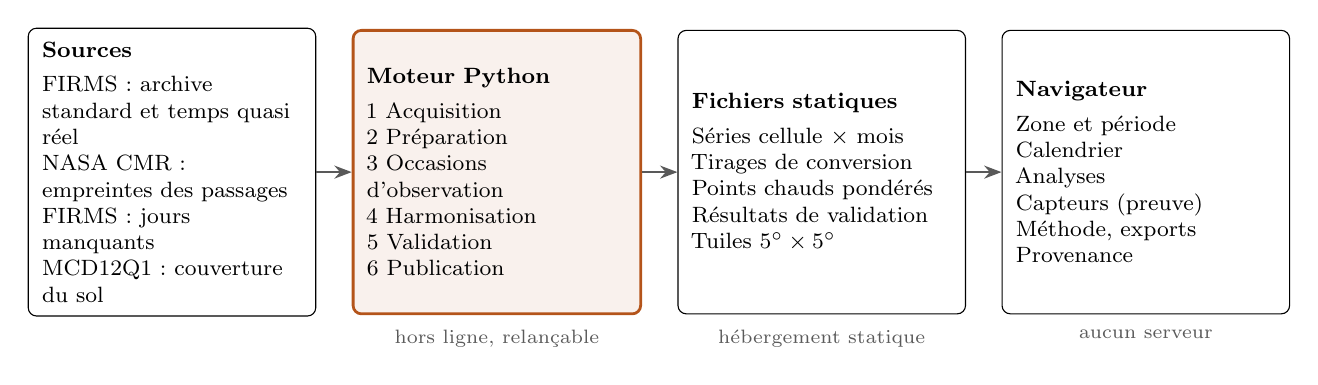
\begin{tikzpicture}[
  box/.style={draw,rounded corners=3pt,align=left,font=\footnotesize,minimum height=3.6cm,text width=3.3cm,inner sep=5pt,execute at begin node=\raggedright},
  arr/.style={-{Stealth[length=2.2mm]},thick,gray!70!black},
  node distance=0.45cm]
  \node[box] (src) {\textbf{Sources}\\[3pt]FIRMS~: archive standard et temps quasi réel\\NASA CMR~: empreintes des passages\\FIRMS~: jours manquants\\MCD12Q1~: couverture du sol};
  \node[box,right=of src,draw=accent,fill=accent!8,line width=1pt] (eng) {\textbf{Moteur Python}\\[3pt]1 Acquisition\\2 Préparation\\3 Occasions d'observation\\4 Harmonisation\\5 Validation\\6 Publication};
  \node[box,right=of eng] (fil) {\textbf{Fichiers statiques}\\[3pt]Séries cellule $\times$ mois\\Tirages de conversion\\Points chauds pondérés\\Résultats de validation\\Tuiles $5^\circ \times 5^\circ$};
  \node[box,right=of fil] (web) {\textbf{Navigateur}\\[3pt]Zone et période\\Calendrier\\Analyses\\Capteurs (preuve)\\Méthode, exports\\Provenance};
  \draw[arr] (src) -- (eng);
  \draw[arr] (eng) -- (fil);
  \draw[arr] (fil) -- (web);
  \node[below=2pt of eng,font=\scriptsize,quiet] {hors ligne, relançable};
  \node[below=2pt of fil,font=\scriptsize,quiet] {hébergement statique};
  \node[below=2pt of web,font=\scriptsize,quiet] {aucun serveur};
\end{tikzpicture}
\caption{Architecture de HEXAFIRE. Chaque étape lit et écrit des fichiers, ce qui permet de reprendre la chaîne à tout moment.}
\label{fig:archi}
\end{figure}

\begin{table}[h]
\centering\small
\caption{Choix technologiques.}
\begin{tabularx}{\linewidth}{l Y}
\toprule
Composant & Technologie \\
\midrule
Moteur & Python, pandas, NumPy, PyArrow~; statsmodels pour les modèles linéaires généralisés \\
Géométrie & Intersection de polygones (Shapely ou implémentation de Sutherland--Hodgman) \\
Stockage intermédiaire & Parquet compressé \\
Fichiers servis & Tableaux typés compressés, tuiles de $5^\circ \times 5^\circ$, moins de 2~Mo par tuile \\
Interface & Vite, React, TypeScript~; MapLibre GL JS~; Observable Plot \\
Hébergement & Statique (GitHub Pages ou Netlify) \\
\bottomrule
\end{tabularx}
\end{table}

\subsection{Algorithmes}

Les algorithmes~\ref{alg:occ} à \ref{alg:zone} décrivent les quatre traitements principaux.

\begin{algorithm}[h]
\caption{Occasions d'observation}
\label{alg:occ}
\begin{algorithmic}[1]
\Require granules CMR (empreinte $P_g$, horaire, plateforme, orbite, jour/nuit)~; jours manquants~; grille de cellules $C_c$
\Ensure $E_{s,c,m,d}$, $E^{\text{ref}}_{c,k,d}$, couverture $\kappa_{c,m}$, statut
\ForAll{plateforme $s$}
  \State regrouper les granules en passages $o$ par numéro d'orbite, sinon par continuité temporelle
  \ForAll{passage $o$}
    \If{le jour de $o$ est manquant pour $s$} \State \textbf{continuer} \EndIf
    \State $U \gets \bigcup_{g\in o} P_g$~; \; $\mathcal{C} \gets$ cellules dont la boîte intersecte celle de $U$
    \ForAll{$c \in \mathcal{C}$}
      \State $E_{s,c,m(o),d(o)} \mathrel{+}= \Aire(C_c \cap U)/\Aire(C_c)$ \Comment{repli~: $+1$ si le centre de $c$ est dans $U$}
    \EndFor
  \EndFor
\EndFor
\State $E^{\text{ref}}_{c,k,d} \gets \med_{y=2003}^{2020} E_{M,c,(y,k),d}$~; calculer $\kappa_{c,m}$ et le statut
\State vérifier qu'au moins 99\,\% des détections tombent dans l'empreinte d'un passage de leur capteur
\end{algorithmic}
\end{algorithm}

\begin{algorithm}[h]
\caption{Estimation de la conversion VIIRS $\to$ MODIS}
\label{alg:conv}
\begin{algorithmic}[1]
\Require comptages $N$ et occasions $E$ par cellule, mois et période~; strates $r(c)$~; période de calibration $\mathcal{C}$
\Ensure $\tilde\alpha_{p,r,k,d}$, $\gamma_{r,k,d}$, paramètres de linéarité
\ForAll{période $d$, plateforme $p = S$}
  \State $\mathcal{D} \gets \{(c,m) \in \mathcal{C}~: \kappa_M \ge 0{,}8,\ \kappa_p \ge 0{,}8,\ n = N_M + N_p \ge 1\}$
  \State ajuster $\logit \pi = \alpha_{r,k} + \log(E_p/E_M)$ par quasi-binomiale sur $\mathcal{D}$ $\Rightarrow$ $\hat\alpha_{r,k}, \sigma_{r,k}$
  \State ajuster $\alpha_r$ (toutes saisons)~; estimer $\hat\tau_r^2$ (DerSimonian--Laird)
  \State $\tilde\alpha_{r,k} \gets w_{r,k}\hat\alpha_{r,k} + (1-w_{r,k})\hat\alpha_r$
  \State contrôle de linéarité~: si l'IC à 95\,\% de $b_r$ exclut 1, conversion non linéaire pour $r$
\EndFor
\State estimer $\delta_{N20,S}$ puis $\delta_{N21,N20}$ par la même régression~; $\tilde\alpha_{N20} \gets \tilde\alpha_S + \delta_{N20,S}$, etc.
\State estimer $\gamma_{r,k,d}$ (Terra face à Terra et Aqua, 2003--2020)
\end{algorithmic}
\end{algorithm}

\begin{algorithm}[h]
\caption{Série harmonisée, poids et tirages}
\label{alg:serie}
\begin{algorithmic}[1]
\Require sorties des algorithmes~\ref{alg:occ} et \ref{alg:conv}~; détections préparées~; $B=200$
\Ensure tables \texttt{harmonized\_cell\_month}, \texttt{hotspots\_weighted}, \texttt{conversion\_draws}
\ForAll{cellule $c$, mois $m$, période $d$}
  \State choisir la source selon la période (tableau~\ref{tab:serie})~; calculer $\hat N_{c,m,d}$ et le statut
  \ForAll{détection $i$ de $(c,m,d)$} \State $w_i \gets$ poids de la section~\ref{sec:poids} \EndFor
  \State contrôler $\left|\sum_i w_i - \hat N_{c,m,d}\right| < 10^{-9}$
\EndFor
\For{$b = 1$ \textbf{à} $B$}
  \State tirer avec remise des années de calibration (blocs d'un an)~; refaire l'algorithme~\ref{alg:conv} $\Rightarrow$ $\tilde\alpha^{(b)}, \gamma^{(b)}$
  \State enregistrer les tirages dans \texttt{conversion\_draws}
\EndFor
\State estimer $\varphi_r$~; découper les tables en tuiles de $5^\circ\times5^\circ$~; publier avec \texttt{metadata.json}
\end{algorithmic}
\end{algorithm}

\begin{algorithm}[h]
\caption{Calendrier d'une zone (exécuté dans le navigateur)}
\label{alg:zone}
\begin{algorithmic}[1]
\Require zone $Z$ (polygone)~; période~; tuiles intersectées
\Ensure calendrier, intervalles, indicateurs, statuts
\State $\mathcal{Z} \gets$ cellules dont le centre est dans $Z$ \Comment{boîte englobante, puis lancer de rayon}
\ForAll{mois $m$ de la période}
  \State $\hat N_{Z,m} \gets \sum_{c\in\mathcal{Z}} \hat N_{c,m}$ sur les cellules observées~; statut de zone (règle des 20\,\%)
  \If{$m$ est converti}
    \For{$b=1$ \textbf{à} $B$} \State $\mu_Z^{(b)} \gets \sum_c \hat N^{(b)}_{c,m}$~; tirer $N_Z^{\ast(b)} \sim \mathrm{NB}(\mu_Z^{(b)},\varphi_Z)$ \EndFor
    \State intervalle $\gets$ quantiles 2,5\,\% et 97,5\,\%
  \EndIf
\EndFor
\State calculer médiane, moyenne, $A$, classe, rang, $P_{Z,m}$~; appliquer les règles de refus
\State \Return calendrier et indicateurs~; convertir en équivalent VIIRS si l'utilisateur le demande
\end{algorithmic}
\end{algorithm}

%====================================================================
\section{Validation}\label{sec:validation}
%====================================================================

\subsection{Objectifs et principes}

La validation répond à trois questions~: la méthode est-elle fiable, est-elle meilleure que l'existant, et d'où vient le gain ? Elle obéit à deux exigences. La première est le \emph{préenregistrement} (V1)~: critère principal, critères secondaires, seuils et découpage des données sont fixés et publiés dans le dépôt avant l'ouverture des jeux de test, et un résultat défavorable est publié tel quel. La seconde est la \emph{séparation} (V2)~: aucun choix de modèle, de filtre ou de seuil n'est fait en regardant les jeux de test, et le chiffre communiqué est celui du test, jamais celui de la calibration.

\subsection{Partition des données}

Le tableau~\ref{tab:partition} donne la partition proposée pour une couverture africaine avec zone témoin. Elle sera adaptée si la couverture mondiale est retenue (section~\ref{sec:plan}).

\begin{table}[h]
\centering\small
\caption{Partition des données (proposition pour la couverture africaine).}
\label{tab:partition}
\begin{tabularx}{\linewidth}{l Y}
\toprule
Usage & Données \\
\midrule
Calibration & Suomi NPP et MODIS, 2012--2017, Afrique de l'Ouest \\
Référence des verdicts & MODIS, 2003--2011, mêmes régions \\
Test temporel & 2018--2020, Afrique de l'Ouest \\
Test spatial & Afrique australe, ouverte une seule fois \\
Test difficile & Zone témoin en Amérique du Nord, avec feux actifs Landsat \\
Test de dérive & 2021--2024, jamais utilisé pour calibrer la méthode finale \\
\bottomrule
\end{tabularx}
\end{table}

Une fois les tests terminés, la méthode retenue est recalibrée sur 2012--2020, mais les résultats publiés restent ceux des tests.

\subsection{Critère principal}

Pour chaque strate $r$ et chaque mois $m$ de la période de test, on compare deux verdicts~: $V^M_{r,m}$, calculé à partir du comptage MODIS réel, et $V^H_{r,m}$, calculé à partir de VIIRS converti, comme si MODIS n'existait plus. Un verdict vaut \og bas\fg, \og normal\fg{} ou \og haut\fg, selon que la valeur est inférieure au centile 10, comprise entre les centiles 10 et 90, ou supérieure au centile 90 des mêmes mois de 2003--2011. Le critère principal est le coefficient $\kappa$ de Cohen~\cite{cohen1960} entre $V^M$ et $V^H$ sur le test temporel~:
\begin{equation}
  \kappa = \frac{p_o - p_e}{1 - p_e},
\end{equation}
où $p_o$ est la proportion d'accord observée et $p_e$ la proportion attendue par hasard. On mesure en complément le taux de fausses anomalies $FA = \Pr(V^H \neq \text{normal} \mid V^M = \text{normal})$.

\subsection{Critères secondaires}

Les mesures portent sur les couples strate-mois du jeu de test, avec l'erreur logarithmique $e_{r,m} = \log(1+\hat N^H_{r,m}) - \log(1+\hat N^M_{r,m})$, où $\hat N^M$ est la valeur MODIS ramenée à l'exposition de référence. La colonne \og Priorité\fg{} indique ce qui est exécuté pendant le hackathon (H) et ce qui est reporté (A).

\begin{longtable}{>{\raggedright\arraybackslash}p{0.8cm} >{\raggedright\arraybackslash}p{2.8cm} >{\raggedright\arraybackslash}p{5.2cm} >{\raggedright\arraybackslash}p{3.8cm} c}
\caption{Tests de validation.}\label{tab:tests}\\
\toprule
N° & Question & Mesure & Valeur cible & Priorité \\
\midrule\endfirsthead
\toprule
N° & Question & Mesure & Valeur cible & Priorité \\
\midrule\endhead
\small T1 & \small Verdict stable ? & \small $\kappa$ et $FA$ (critère principal) & \small $\kappa \ge 0{,}5$ et $FA \le 0{,}15$ & H \\
\small T2 & \small Valeurs exactes ? & \small Biais $\med(e)$, erreur $\med|e|$ & \small $|\med(e)| < 0{,}10$, $\med|e| < 0{,}25$ & H \\
\small T3 & \small Intervalles honnêtes ? & \small Part des valeurs MODIS dans l'intervalle à 95\,\% & \small entre 90\,\% et 98\,\% & H \\
\small T4 & \small Pas de marche ? & \small Moyenne de $e$ après une bascule fictive en 2015, 2016 ou 2017 & \small $|\bar e| < 0{,}10$, intervalle contenant 0 & H \\
\small T5 & \small Variabilité préservée ? & \small Rapport des variances interannuelles, corrélation des anomalies & \small rapport entre 0,8 et 1,25~; $r \ge 0{,}8$ & A \\
\small T6 & \small Mois extrêmes ? & \small Biais sur le décile supérieur des mois MODIS & \small pas pire que T2, sinon conversion non linéaire & A \\
\small T7a & \small Procédure transférable ? & \small Calibration et test locaux dans une autre région & \small mêmes cibles que T1 et T2 & A \\
\small T7b & \small Conversion transférable ? & \small Conversion appliquée sans recalibrage, par classe de couverture du sol & \small erreur au plus 1,5 fois celle de T2 & A \\
\small T8 & \small Zone témoin & \small Accord avec les anomalies Landsat & \small rapporté, sans seuil & A \\
\small T9 & \small Dérive après 2020 ? & \small Tendance du rapport MODIS sur VIIRS, 2021--2024 & \small bascule avancée si dérive significative dès 2020 & H \\
\small T10 & \small Flux récent comparable ? & \small Rapport flux récent sur archive, mêmes mois & \small stable, sinon facteur correctif & A \\
\small T11 & \small Référence externe & \small Corrélation de Spearman avec les anomalies de surface brûlée & \small $\rho \ge 0{,}6$ en savane, supérieure au raccord brut & A \\
\small T12 & \small Fuite d'information ? & \small Performance après permutation des années & \small doit s'effondrer & A \\
\small T13 & \small Chaînage fiable ? & \small Écart entre $\alpha_{N20}$ chaîné et estimé directement sur 2018--2020 & \small dans l'intervalle à 95\,\% & A \\
\bottomrule
\end{longtable}

\paragraph{Marche à la bascule réelle.} Sur la série harmonisée agrégée par strate, on ajuste
\begin{equation}
  \log(1 + \hat N_{r,m}) = \beta_0 + \sum_k \beta_k \mathbf{1}\{k(m) = k\} + \beta_t\, t_m + \delta\, \mathbf{1}\{m \ge m^\ast\} + \varepsilon_m,
\end{equation}
avec des erreurs autorégressives d'ordre 1 et $m^\ast$ = janvier 2021. La marche $\delta$ est rapportée avec son intervalle de confiance. Elle est interprétée avec prudence, car elle peut aussi refléter un changement réel d'activité.

\subsection{Expériences sur données simulées}

Les données réelles ne fournissent pas l'activité vraie, alors qu'un banc d'essai simulé la fournit. L'activité vraie est générée par $\lambda_{c,m} = \lambda_c\, s_{c,k}\, u_{c,y}\, \varepsilon_{c,m}$, avec un cycle saisonnier $s$, un facteur annuel $u$ incluant quelques années extrêmes, et un bruit log-normal. Les comptages sont ensuite tirés selon les équations~\eqref{eq:nbM} et \eqref{eq:nbP}, à partir des occasions et des jours manquants réels. Plusieurs scénarios de défaut sont simulés~: relation non linéaire, dérive de l'heure de passage, sensibilité différente selon la région, lacunes prolongées. Chaque méthode doit retrouver les verdicts calculés sur l'activité vraie. Ce test est le seul où la vérité est connue, mais il ne vaut que pour les mécanismes simulés.

\subsection{Analyse d'ablation et de sensibilité}\label{sec:ablation}

Chaque composant est retiré à tour de rôle, puis la méthode est réévaluée sur T1 et T2. Les variantes testées sont les suivantes~: sans occasions d'observation ($E\equiv1$), sans effet du mois de l'année, sans strates, sans stabilisation, sans distinction jour/nuit, sans bascule en 2021, avec relation non linéaire, et avec ou sans filtres de confiance. Un composant qui n'améliore aucun critère est retiré de la méthode finale. La sensibilité est évaluée de plusieurs façons~: fenêtres de calibration décalées (2012--2016, 2014--2018), grilles de $0{,}25^\circ$ et $0{,}5^\circ$, détections de jour seules, de nuit seules ou réunies, et suppression des doublons. Une méthode est jugée robuste si $\kappa$ varie de moins de 0,1 entre ces variantes.

\subsection{Contrôles d'intégrité}

Les contrôles suivants sont automatiques~:
\begin{itemize}
  \item conservation~: la somme des comptages par cellule égale le nombre de lignes retenues~;
  \item poids~: $\sum_i w_i = \hat N_{c,m}$ à $10^{-9}$ près~;
  \item occasions~: chaque terme de l'équation~\eqref{eq:occasions} est compris entre 0 et 1, et l'exigence des 99\,\% est respectée~;
  \item jours manquants~: un jour signalé manquant donne une contribution nulle pour le capteur concerné~;
  \item reproductibilité~: deux exécutions identiques donnent des fichiers identiques au bit près~;
  \item export~: un CSV réimporté redonne les valeurs affichées.
\end{itemize}

%====================================================================
\section{Comparaison aux méthodes existantes}\label{sec:comparaison}
%====================================================================

HEXAFIRE (H) est comparé aux méthodes M0 à M6 de la section~\ref{sec:methodes}, réimplémentées sur exactement les mêmes données, filtres et découpages. Le protocole est le suivant.
\begin{enumerate}
  \item Pour chaque méthode et chaque couple strate-mois du jeu de test, on calcule une perte~: le désaccord de verdict pour le critère principal, $|e_{r,m}|$ pour l'exactitude.
  \item La différence de performance entre HEXAFIRE et une méthode de référence est calculée sur les mêmes couples, ce qui en fait une comparaison appariée.
  \item Son intervalle de confiance à 95\,\% est obtenu par rééchantillonnage des années avec $B = 2\,000$ tirages~\cite{efron1993}.
  \item Une seule comparaison est confirmatoire~: HEXAFIRE contre M2 sur le critère principal. Les autres sont descriptives, ce qui évite les conclusions dues aux tests multiples.
\end{enumerate}
HEXAFIRE est déclaré supérieur à M2 si l'intervalle de confiance à 95\,\% de $\kappa_H - \kappa_{M2}$ est entièrement positif et si aucun critère T2 à T5 ne se dégrade au-delà de sa cible. Les règles de décision sont fixées à l'avance (tableau~\ref{tab:decision}).

\begin{table}[h]
\centering\small
\caption{Règles de décision.}
\label{tab:decision}
\begin{tabularx}{\linewidth}{Y Y}
\toprule
Résultat & Décision \\
\midrule
H supérieur à M2, T1 à T5 atteints & H est la méthode de l'application \\
H équivalent à M2, T1 à T5 atteints & M2 est retenue pour sa simplicité~; H est conservé pour l'incertitude et le statut d'observation \\
T6 non atteint & Conversion non linéaire~; si l'échec persiste, les mois extrêmes sont signalés \\
T4 ou T5 non atteint & La série n'est pas présentée comme harmonisée \\
T1 non atteint pour toutes les méthodes & Capteurs affichés séparément avec l'anomalie par capteur, et échec publié \\
T10 non atteint & Le mois en cours est marqué \og non comparable\fg \\
\bottomrule
\end{tabularx}
\end{table}

Si la règle de supériorité est satisfaite, l'affirmation publiée prend la forme suivante~: \og Sur des années et une région non utilisées pour la calibration, la méthode HEXAFIRE réduit le désaccord de verdict entre capteurs de X\,\% par rapport au ratio régional, sans lisser la variabilité interannuelle.\fg{} Aucune affirmation n'est faite en dehors des régions et des périodes testées.

%====================================================================
\section{Application web}\label{sec:appli}
%====================================================================

L'application comporte cinq onglets et un panneau de provenance accessible depuis chaque valeur. La zone et la période choisies sont conservées d'un onglet à l'autre. L'application s'ouvre dans un navigateur, sur ordinateur comme sur téléphone, sans installation.

\begin{table}[h]
\centering\small
\caption{Onglets de l'application.}
\begin{tabularx}{\linewidth}{>{\raggedright\arraybackslash}p{2.6cm} Y >{\raggedright\arraybackslash}p{2cm}}
\toprule
Onglet & Contenu & Exigences \\
\midrule
1. Zone & Carte, tracé de rectangle, polygone ou point avec rayon~; saisie de coordonnées~; période~; résumé des cellules retenues & E4, E5 \\
2. Calendrier & Grille années $\times$ mois~; quatre indicateurs (activité du mois et marge, écart à la médiane, rang, couverture)~; modes \og niveau d'activité\fg{} (palette séquentielle) et \og écart à la normale\fg{} (palette divergente)~; unité équivalent MODIS ou VIIRS~; statut par texture & E2, E3, E8, E15 \\
3. Analyses & Mois en cours face à l'historique~; profil saisonnier~; classement des années~; saison cumulée~; épisode en cours~; mois les plus inhabituels, triés par fiabilité & E9 à E13 \\
4. Capteurs & Détections brutes par capteur~; rapportées aux occasions~; commutateur brut/harmonisé~; anomalie par capteur~; fiches des satellites~; résultats du banc d'essai & E1, E16 \\
5. Méthode et exports & Fiches explicatives~; CSV du calendrier, des points chauds pondérés et des analyses~; figures PNG et SVG~; métadonnées & E6, E7, E14 \\
\bottomrule
\end{tabularx}
\end{table}

\paragraph{Statuts des cases.} La couleur porte la valeur et une texture porte le statut, ce qui reste lisible en noir et blanc et pour les personnes daltoniennes. Six statuts sont distingués~:
\begin{itemize}
  \item \emph{mesuré}~: couleur pleine~;
  \item \emph{converti}~: couleur pleine et petit triangle~;
  \item \emph{aucun point chaud}~: couleur la plus claire et point central~;
  \item \emph{couverture partielle}~: hachures légères~;
  \item \emph{non observé}~: hachures sans couleur~;
  \item \emph{données manquantes}~: case vide à contour pointillé.
\end{itemize}
En mode \og écart à la normale\fg, deux mentions s'ajoutent~: \og référence insuffisante\fg{} et \og effectif trop faible\fg.

\paragraph{Démonstration principale.} Le commutateur \og brut / harmonisé\fg{} de l'onglet Capteurs montre que la marche visible au changement de capteur disparaît, sans que les variations d'une année à l'autre soient effacées.

\paragraph{Accessibilité.} L'application respecte le niveau de contraste AA des recommandations WCAG, se navigue au clavier et fournit des textes alternatifs pour les figures. Sur téléphone, le calendrier pivote. L'interface est disponible en français et en anglais.

\paragraph{Données produites.} Le moteur publie six tables et un fichier de métadonnées~:
\begin{itemize}
  \item \texttt{cell\_month}~: comptages et occasions par cellule, mois et capteur~;
  \item \texttt{harmonized\_cell\_month}~: $\hat N$, source, $E^{\text{ref}}$, couverture et statut~;
  \item \texttt{conversion\_draws}~: tirages de $\tilde\alpha$, $\gamma$, $a$ et $b$~;
  \item \texttt{dispersion}~: $\varphi_r$~;
  \item \texttt{hotspots\_weighted}~: détections avec leur poids~;
  \item \texttt{validation\_results}~: résultats des tests~;
  \item \texttt{metadata.json}~: versions, empreintes et paramètres.
\end{itemize}
Les exigences de qualité portent sur la reproductibilité (versions figées, graine fixée, commande unique) et la traçabilité (empreinte SHA-256 de chaque source). Elles fixent aussi des performances~: recalibration en moins de 10 minutes, tuile de moins de 2~Mo, calendrier affiché en moins de 2 secondes. Enfin, aucune clé d'accès ne doit apparaître dans les fichiers publiés, et le code doit être ouvert.

%====================================================================
\section{Plan de réalisation et décisions ouvertes}\label{sec:plan}
%====================================================================

\subsection{Priorités pour le hackathon (14--15 novembre 2026)}

Le périmètre complet décrit ci-dessus dépasse ce que deux jours permettent. Les priorités sont les suivantes.
\begin{enumerate}
  \item \textbf{Indispensable.} Acquisition FIRMS et préparation (P1--P9). Occasions d'observation par la méthode de repli. Conversion par régression logistique, avec jour/nuit et stabilisation. Série, poids et statuts. Tests T1 à T4 et T9, et comparaison à M0, M2 et M5. Onglets Zone, Calendrier et exports.
  \item \textbf{Souhaitable.} Calcul géométrique exact des occasions. Intervalles de prédiction dans le navigateur. Onglets Analyses et Capteurs complets.
  \item \textbf{Après le hackathon.} Tests T5 à T8 et T10 à T13. Banc simulé. Ablation complète. Comparaison à M1, M3, M4 et M6. Zone témoin Landsat.
\end{enumerate}

\subsection{Couverture géographique}

\begin{decision}{Décision du 12 novembre 2026}
L'équipe retient l'option~B~: \textbf{monde entier}. Les strates sont provisoirement des blocs de $10^\circ$, en attendant les régions GFED croisées avec l'occupation du sol.
\end{decision}

Les deux options examinées étaient les suivantes.
\begin{description}[leftmargin=0.6cm,style=nextline]
  \item[Option A~: Afrique et zone témoin en Amérique du Nord.] Le volume de données est maîtrisé et la partition de validation du tableau~\ref{tab:partition} est déjà définie. Une vérification indépendante est possible par Landsat. En revanche, l'application ne répond pas à un utilisateur hors de ces régions.
  \item[Option B~: monde entier.] L'application répond à tout utilisateur, conformément à l'esprit du défi. Les strates s'appuient sur les quatorze régions GFED. En revanche, le volume de données et le temps de calcul des occasions sont bien plus élevés, et la partition de validation doit être étendue (test spatial sur un autre continent).
\end{description}
Une voie intermédiaire consiste à valider sur l'Afrique et la zone témoin, puis à appliquer la méthode au monde entier en le signalant comme \og non validé hors des régions testées\fg.

%====================================================================
\section{Limites et discussion}\label{sec:discussion}
%====================================================================

\paragraph{Résultats (provisoires).} La chaîne a été exécutée sur le monde entier avec MODIS (novembre~2000--juin~2024) et S-NPP (2012--2020). Les archives proviennent du serveur de l'équipe feux de l'université du Maryland, qui distribue les produits NASA. À passages égaux, en médiane des 328~strates, un point chaud S-NPP vaut 0,185 point chaud MODIS de jour (soit VIIRS $\approx 5{,}4\times$ MODIS) et 0,064 de nuit ($\approx 15{,}6\times$). Ces valeurs viennent d'une première calibration sur 2012--2013. La validation \og une année exclue\fg{} sur 2012--2015 compare 7\,604 strates-mois~:

\begin{center}\small
\begin{tabular}{lccccc}
\toprule
Méthode & $\kappa$ & Fausses anomalies & Biais & Erreur & Marche \\
\midrule
HEXAFIRE & \textbf{0,735} & \textbf{0,098} & \textbf{0,014} & \textbf{0,127} & \textbf{0,051} \\
M1 (facteur global) & 0,553 & 0,239 & 0,045 & 0,255 & 0,123 \\
M0 (raccord brut) & 0,015 & 0,925 & 1,962 & 1,962 & 2,028 \\
\midrule
Cible & $\geq 0{,}5$ & $\leq 0{,}15$ & $|\cdot|<0{,}10$ & $<0{,}25$ & $<0{,}10$ \\
\bottomrule
\end{tabular}
\end{center}

HEXAFIRE atteint les cinq cibles. L'intervalle de confiance à 95\,\% de $\kappa_H-\kappa_{M1}$, obtenu par rééchantillonnage des années, vaut $[0{,}168~;~0{,}195]$ et ne contient pas zéro. Ces chiffres seront mis à jour avec la calibration sur 2012--2020 complet et S-NPP 2021--2026. Le détail des modèles tels qu'ils sont implantés figure dans le dossier technique de l'application.

\paragraph{Limites.} Un point chaud n'est pas un incendie~: un grand feu produit de nombreuses détections, et beaucoup de petits feux ne sont jamais détectés. Les nuages et la fumée masquent une partie des feux, et avec les seules données FIRMS un mois nuageux et un mois sans feu ne se distinguent pas entièrement. Les valeurs converties sont des estimations, dont la marge est affichée. VIIRS n'a pas de passage en milieu de matinée équivalent à celui de Terra, et la conversion suppose une relation stable entre capteurs, testée par région. La période de novembre 2000 à juin 2002 repose sur Terra seul et présente une incertitude plus large. La grille de $0{,}25^\circ$ rend les très petites zones imprécises. Enfin, les feux signalés au sol ne sont pas intégrés, faute de données homogènes.

\paragraph{Discussion.} Les deux versions préalables de ce travail divergeaient sur le sens de la conversion. La première convertissait MODIS en équivalent VIIRS, la seconde VIIRS en équivalent MODIS. Le choix de MODIS comme unité de calcul est retenu pour trois raisons. Il ne reconstitue pas le passé, il s'appuie sur une référence mesurée de dix-huit ans, et il rend la méthode directement testable. Il suit aussi la pratique des travaux récents~\cite{chen2026,li2020,seguini2026}. Comme les anomalies sont invariantes au changement d'unité lorsque la conversion est proportionnelle, l'affichage en équivalent VIIRS reste offert sans coût scientifique. La première version apporte au modèle retenu la distinction du jour et de la nuit, une revue élargie des méthodes et de la littérature, et l'idée de stabiliser les petites strates vers une valeur régionale. La seconde apporte les occasions d'observation, l'estimation conditionnelle, le critère d'invariance du verdict et le protocole de comparaison.

%====================================================================
\section{Conclusion}
%====================================================================

HEXAFIRE harmonise l'archive des points chauds MODIS et VIIRS en exprimant VIIRS dans l'unité de MODIS, à occasions d'observation égales. La conversion est estimée par une régression logistique conditionnelle stratifiée, qui élimine l'activité inconnue et traite les deux capteurs symétriquement. Chaque valeur est assortie d'un intervalle de prédiction et d'un statut d'observation, et chaque détection porte un poids harmonisé. La méthode est jugée sur le critère même du défi, l'invariance du verdict, mesurée sur des données réservées et comparée à six méthodes existantes. L'application statique qui en découle permet à tout utilisateur de lire, pour sa zone, quand surviennent les feux, quelles années ont été exceptionnelles et comment le mois en cours se situe par rapport au passé.

%====================================================================
\begin{thebibliography}{99}
\small

\bibitem[Boschetti et al.(2022)]{boschetti2022}
L.~Boschetti, D.~P. Roy et L.~Giglio.
\newblock Is the world burning less? Harmonization of the NASA MODIS and VIIRS fire product record.
\newblock Présentation, NASA MODIS Science Team Meeting, 2022.

\bibitem[Chen et al.(2023)]{chen2023}
Y.~Chen, J.~Hall, D.~van~Wees, N.~Andela, S.~Hantson, L.~Giglio, G.~R. van~der Werf, D.~C. Morton et J.~T. Randerson.
\newblock Multi-decadal trends and variability in burned area from the fifth version of the Global Fire Emissions Database (GFED5).
\newblock \emph{Earth System Science Data}, 15:5227--5259, 2023.

\bibitem[Chen et al.(2026)]{chen2026}
Y.~Chen, G.~R. van~der Werf, M.~Mu, D.~van~Wees, J.~V. Hall, L.~Giglio et al.
\newblock Tracking recent extremes and interannual variability of global fire emissions using a near-real-time extension to the Global Fire Emissions Database.
\newblock \emph{Earth System Science Data}, 18:7535--7555, 2026. doi:10.5194/essd-18-7535-2026.

\bibitem[Cohen(1960)]{cohen1960}
J.~Cohen.
\newblock A coefficient of agreement for nominal scales.
\newblock \emph{Educational and Psychological Measurement}, 20(1):37--46, 1960.

\bibitem[DerSimonian et Laird(1986)]{dersimonian1986}
R.~DerSimonian et N.~Laird.
\newblock Meta-analysis in clinical trials.
\newblock \emph{Controlled Clinical Trials}, 7(3):177--188, 1986.

\bibitem[NASA Earthdata(2026)]{earthdata2026}
NASA Earthdata.
\newblock Transitioning from Suomi NPP VIIRS \& OMPS: what FIRMS users need to know, 2026.
\newblock \url{https://www.earthdata.nasa.gov/news/blog/transitioning-from-suomi-npp-viirs-omps-what-firms-users-need-know}

\bibitem[Efron et Tibshirani(1993)]{efron1993}
B.~Efron et R.~J. Tibshirani.
\newblock \emph{An Introduction to the Bootstrap}.
\newblock Chapman \& Hall, 1993.

\bibitem[FIRMS(2026a)]{firms}
NASA FIRMS.
\newblock Fire Information for Resource Management System --- Archive Download.
\newblock \url{https://firms.modaps.eosdis.nasa.gov/download/}, consulté le 11 novembre 2026.

\bibitem[FIRMS(2026b)]{firmsmissing}
NASA FIRMS.
\newblock Missing data table.
\newblock \url{https://firms.modaps.eosdis.nasa.gov/api/missing_data/}

\bibitem[Fu et al.(2020)]{fu2020}
Y.~Fu, R.~Li, X.~Wang, Y.~Bergeron, O.~Valeria, R.~D. Chavardès, Y.~Wang et J.~Hu.
\newblock Fire detection and fire radiative power in forests and low-biomass lands in Northeast Asia: MODIS versus VIIRS fire products.
\newblock \emph{Remote Sensing}, 12(18):2870, 2020.

\bibitem[Giglio et al.(2006)]{giglio2006}
L.~Giglio, G.~R. van~der Werf, J.~T. Randerson, G.~J. Collatz et P.~Kasibhatla.
\newblock Global estimation of burned area using MODIS active fire observations.
\newblock \emph{Atmospheric Chemistry and Physics}, 6:957--974, 2006.

\bibitem[Giglio et al.(2025)]{giglio2025}
L.~Giglio, L.~Boschetti, D.~P. Roy, J.~V. Hall, M.~Zubkova, M.~Humber, H.~Huang et V.~Oles.
\newblock The NASA VIIRS burned area product, global validation, and intercomparison with the NASA MODIS burned area product.
\newblock \emph{Remote Sensing of Environment}, 331:115006, 2025.

\bibitem[Kaiser et al.(2012)]{kaiser2012}
J.~W. Kaiser, A.~Heil, M.~O. Andreae, A.~Benedetti, N.~Chubarova, L.~Jones et al.
\newblock Biomass burning emissions estimated with a global fire assimilation system based on observed fire radiative power.
\newblock \emph{Biogeosciences}, 9:527--554, 2012.

\bibitem[Künsch(1989)]{kunsch1989}
H.~R. Künsch.
\newblock The jackknife and the bootstrap for general stationary observations.
\newblock \emph{The Annals of Statistics}, 17(3):1217--1241, 1989.

\bibitem[Li et al.(2018)]{li2018}
F.~Li, X.~Zhang, S.~Kondragunta et I.~Csiszar.
\newblock Comparison of fire radiative power estimates from VIIRS and MODIS observations.
\newblock \emph{Journal of Geophysical Research: Atmospheres}, 123:4545--4563, 2018.

\bibitem[Li et al.(2020)]{li2020}
X.~Li, Y.~Zhou, M.~Zhao et X.~Zhao.
\newblock A harmonized global nighttime light dataset 1992--2018.
\newblock \emph{Scientific Data}, 7, 2020.

\bibitem[NASA Space Apps(2026)]{spaceapps2026}
NASA Space Apps Challenge.
\newblock Harmonization of MODIS and VIIRS Hot Spots --- énoncé du défi, 2026.

\bibitem[NSIDC(2025)]{nsidc}
National Snow and Ice Data Center.
\newblock MODIS data: ongoing changes in Terra and Aqua orbits.
\newblock \url{https://nsidc.org/data/modis}

\bibitem[Schroeder et al.(2014)]{schroeder2014}
W.~Schroeder, P.~Oliva, L.~Giglio et I.~A. Csiszar.
\newblock The new VIIRS 375 m active fire detection data product: algorithm description and initial assessment.
\newblock \emph{Remote Sensing of Environment}, 143:85--96, 2014.

\bibitem[Seguini et al.(2026)]{seguini2026}
L.~Seguini, A.~Klisch, M.~Meroni, A.~Vrieling, G.~Manfron, C.~Atzberger et F.~Rembold.
\newblock Global near real-time 500 m 10 d FPAR dataset from MODIS and VIIRS for operational agricultural monitoring and crop yield forecasting.
\newblock \emph{Earth System Science Data}, 18:309--331, 2026.

\bibitem[van der Werf et al.(2025)]{vanderwerf2025}
G.~R. van~der Werf, J.~T. Randerson, D.~van~Wees, Y.~Chen, L.~Giglio, J.~Hall et al.
\newblock Landscape fire emissions from the 5th version of the Global Fire Emissions Database (GFED5).
\newblock \emph{Scientific Data}, 12:1870, 2025.

\bibitem[Zheng et al.(2026)]{zheng2026}
Y.~Zheng, K.~Ding, L.~Xue, Z.~Wang, G.~Jiao, Y.~Zhu, J.~Zhang et Q.~Ren.
\newblock Fire radiative power correction and spatiotemporal fusion based on MYD14 and VNP14IMG.
\newblock \emph{Remote Sensing}, 18(10):1650, 2026.

\end{thebibliography}

\end{document}
